\documentclass{standalone}
\usepackage{tikz}
\usetikzlibrary{patterns, positioning}
\usepackage[sfdefault]{ClearSans} %% option 'sfdefault' activates Clear Sans as the default text font
\usepackage[T1]{fontenc}

\begin{document}
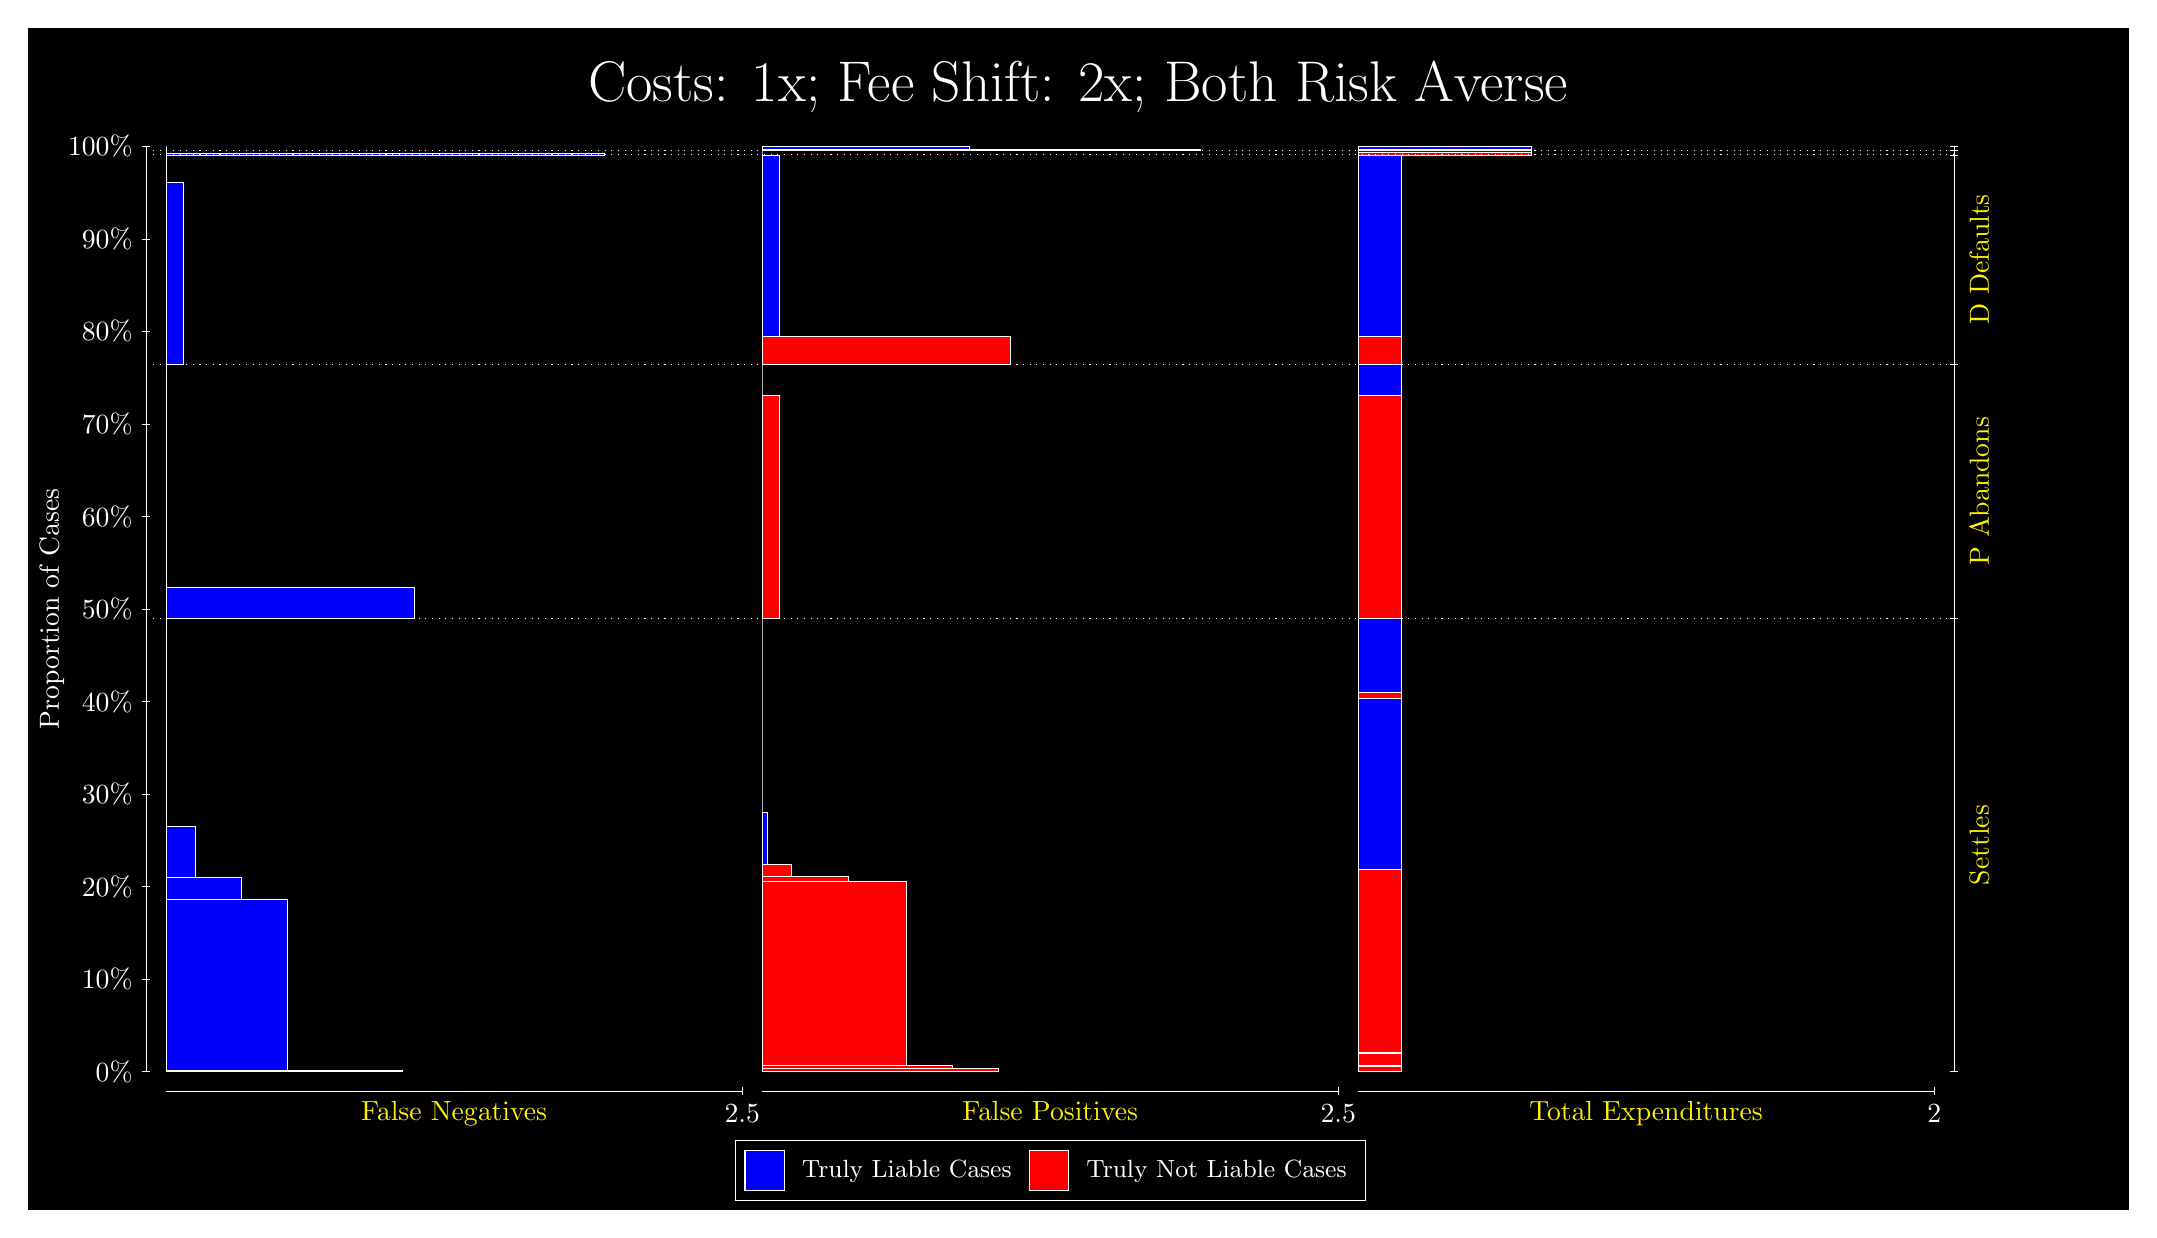
\begin{tikzpicture}
\draw[fill=black] (0,0) rectangle (26.667,15);
\draw[text=white] (0,13.5) rectangle (26.667,15) node[midway] {\huge Costs: 1x; Fee Shift: 2x; Both Risk Averse};
\draw[white, very thin] (1.5,1.75) -- (1.5,13.5);
\node[rotate=90, text=white, anchor=center] at (0.3, 7.625) {Proportion of Cases};
\draw[white, very thin] (1.45,1.75) -- (1.55,1.75);
\node[text=white, anchor=east] at (1.45, 1.75) {0\%};
\draw[white, very thin] (1.45,2.925) -- (1.55,2.925);
\node[text=white, anchor=east] at (1.45, 2.925) {10\%};
\draw[white, very thin] (1.45,4.1) -- (1.55,4.1);
\node[text=white, anchor=east] at (1.45, 4.1) {20\%};
\draw[white, very thin] (1.45,5.275) -- (1.55,5.275);
\node[text=white, anchor=east] at (1.45, 5.275) {30\%};
\draw[white, very thin] (1.45,6.45) -- (1.55,6.45);
\node[text=white, anchor=east] at (1.45, 6.45) {40\%};
\draw[white, very thin] (1.45,7.625) -- (1.55,7.625);
\node[text=white, anchor=east] at (1.45, 7.625) {50\%};
\draw[white, very thin] (1.45,8.8) -- (1.55,8.8);
\node[text=white, anchor=east] at (1.45, 8.8) {60\%};
\draw[white, very thin] (1.45,9.975) -- (1.55,9.975);
\node[text=white, anchor=east] at (1.45, 9.975) {70\%};
\draw[white, very thin] (1.45,11.15) -- (1.55,11.15);
\node[text=white, anchor=east] at (1.45, 11.15) {80\%};
\draw[white, very thin] (1.45,12.325) -- (1.55,12.325);
\node[text=white, anchor=east] at (1.45, 12.325) {90\%};
\draw[white, very thin] (1.45,13.5) -- (1.55,13.5);
\node[text=white, anchor=east] at (1.45, 13.5) {100\%};

\draw[white, very thin] (24.457,1.75) -- (24.457,13.5);
\draw[white, very thin] (24.407,1.75) -- (24.507,1.75);
\node[anchor=west] at (24.407, 1.75) {};
\draw[white, very thin] (24.407,7.5032) -- (24.507,7.5032);
\node[anchor=west] at (24.407, 7.5032) {};
\draw[white, very thin] (24.407,10.732) -- (24.507,10.732);
\node[anchor=west] at (24.407, 10.732) {};
\draw[white, very thin] (24.407,13.392) -- (24.507,13.392);
\node[anchor=west] at (24.407, 13.392) {};
\draw[white, very thin] (24.407,13.445) -- (24.507,13.445);
\node[anchor=west] at (24.407, 13.445) {};
\draw[white, very thin] (24.407,13.5) -- (24.507,13.5);
\node[anchor=west] at (24.407, 13.5) {};

\draw[white, very thin, fill=blue] (1.75,1.75) rectangle (4.7507,1.7597);
\draw[white, very thin, fill=blue] (1.75,1.7597) rectangle (4.0188,1.7694);
\draw[white, very thin, fill=blue] (1.75,1.7694) rectangle (3.4333,1.7695);
\draw[white, very thin, fill=blue] (1.75,1.7695) rectangle (3.287,3.9391);
\draw[white, very thin, fill=blue] (1.75,3.9391) rectangle (2.7015,4.2121);
\draw[white, very thin, fill=blue] (1.75,4.2121) rectangle (2.1159,4.8704);
\draw[white, very thin, fill=red] (1.75,4.8704) rectangle (1.75,7.5032);
\draw[white, very thin, fill=blue] (1.75,7.5032) rectangle (4.8971,7.8958);
\draw[white, very thin, fill=red] (1.75,7.8958) rectangle (1.75,10.732);
\draw[white, very thin, fill=blue] (1.75,10.732) rectangle (1.9696,13.039);
\draw[white, very thin, fill=red] (1.75,13.039) rectangle (1.75,13.392);
\draw[white, very thin, fill=blue] (1.75,13.392) rectangle (7.3123,13.412);
\draw[white, very thin, fill=red] (1.75,13.412) rectangle (1.75,13.445);
\draw[white, very thin, fill=red] (1.75,13.445) rectangle (1.75,13.465);
\draw[white, very thin, fill=blue] (1.75,13.465) rectangle (1.75,13.5);
\draw[white, very thin, fill=red] (9.3189,1.75) rectangle (12.32,1.7903);
\draw[white, very thin, fill=red] (9.3189,1.7903) rectangle (11.734,1.8319);
\draw[white, very thin, fill=red] (9.3189,1.8319) rectangle (11.149,4.1614);
\draw[white, very thin, fill=red] (9.3189,4.1614) rectangle (11.002,4.1615);
\draw[white, very thin, fill=red] (9.3189,4.1615) rectangle (10.417,4.2253);
\draw[white, very thin, fill=red] (9.3189,4.2253) rectangle (9.6848,4.3827);
\draw[white, very thin, fill=blue] (9.3189,4.3827) rectangle (9.3921,5.041);
\draw[white, very thin, fill=blue] (9.3189,5.041) rectangle (9.3189,7.5032);
\draw[white, very thin, fill=red] (9.3189,7.5032) rectangle (9.5384,10.339);
\draw[white, very thin, fill=blue] (9.3189,10.339) rectangle (9.3189,10.732);
\draw[white, very thin, fill=red] (9.3189,10.732) rectangle (12.466,11.085);
\draw[white, very thin, fill=blue] (9.3189,11.085) rectangle (9.5384,13.392);
\draw[white, very thin, fill=red] (9.3189,13.392) rectangle (9.3189,13.426);
\draw[white, very thin, fill=blue] (9.3189,13.426) rectangle (9.3189,13.445);
\draw[white, very thin, fill=red] (9.3189,13.445) rectangle (14.881,13.465);
\draw[white, very thin, fill=blue] (9.3189,13.465) rectangle (11.954,13.5);
\draw[white, very thin, fill=red] (16.888,1.75) rectangle (17.437,1.8138);
\draw[white, very thin, fill=blue] (16.888,1.8138) rectangle (17.437,1.8235);
\draw[white, very thin, fill=red] (16.888,1.8235) rectangle (17.437,1.9809);
\draw[white, very thin, fill=blue] (16.888,1.9809) rectangle (17.437,1.9906);
\draw[white, very thin, fill=red] (16.888,1.9906) rectangle (17.437,4.3202);
\draw[white, very thin, fill=blue] (16.888,4.3202) rectangle (17.437,6.4899);
\draw[white, very thin, fill=red] (16.888,6.4899) rectangle (17.437,6.5719);
\draw[white, very thin, fill=blue] (16.888,6.5719) rectangle (17.437,7.5032);
\draw[white, very thin, fill=red] (16.888,7.5032) rectangle (17.437,10.339);
\draw[white, very thin, fill=blue] (16.888,10.339) rectangle (17.437,10.732);
\draw[white, very thin, fill=red] (16.888,10.732) rectangle (17.437,11.085);
\draw[white, very thin, fill=blue] (16.888,11.085) rectangle (17.437,13.392);
\draw[white, very thin, fill=red] (16.888,13.392) rectangle (19.083,13.426);
\draw[white, very thin, fill=blue] (16.888,13.426) rectangle (19.083,13.445);
\draw[white, very thin, fill=red] (16.888,13.445) rectangle (19.083,13.465);
\draw[white, very thin, fill=blue] (16.888,13.465) rectangle (19.083,13.5);
\draw[white, dotted] (1.5,7.5032) -- (24.457,7.5032);
\draw[white, dotted] (1.5,10.732) -- (24.457,10.732);
\draw[white, dotted] (1.5,13.392) -- (24.457,13.392);
\draw[white, dotted] (1.5,13.445) -- (24.457,13.445);
\draw[white, very thin] (1.75,1.5) -- (9.0689,1.5);
\node[text=yellow, anchor=north] at (5.4094, 1.5) {False Negatives};
\draw[white, very thin] (9.0689,1.45) -- (9.0689,1.55);
\node[text=white, anchor=north] at (9.0689, 1.45) {2.5};

\draw[white, very thin] (9.3189,1.5) -- (16.638,1.5);
\node[text=yellow, anchor=north] at (12.978, 1.5) {False Positives};
\draw[white, very thin] (16.638,1.45) -- (16.638,1.55);
\node[text=white, anchor=north] at (16.638, 1.45) {2.5};

\draw[white, very thin] (16.888,1.5) -- (24.207,1.5);
\node[text=yellow, anchor=north] at (20.547, 1.5) {Total Expenditures};
\draw[white, very thin] (24.207,1.45) -- (24.207,1.55);
\node[text=white, anchor=north] at (24.207, 1.45) {2};

\node[text=yellow, centered, rotate=90] at (24.777, 4.6266) {Settles};
\node[text=yellow, centered, rotate=90] at (24.777, 9.1176) {P Abandons};
\node[text=yellow, centered, rotate=90] at (24.777, 12.062) {D Defaults};



\draw (12.978300999999998,1.5) node[draw=none] (baseCoordinate) {};
\begin{scope}[align=center]
        \matrix[scale=0.5, draw=white, below=0.5cm of baseCoordinate, nodes={draw}, column sep=0.1cm]{
            \node[rectangle, draw, minimum width=0.5cm, minimum height=0.5cm, fill=blue] {}; &
            \node[draw=none, font=\small, text=white] (B) {Truly Liable Cases}; &
            \node[rectangle, draw, minimum width=0.5cm, minimum height=0.5cm, fill=red] {}; &
            \node[draw=none, font=\small, text=white] (B) {Truly Not Liable Cases}; \\
            };
\end{scope}

\end{tikzpicture}
\end{document}